\documentclass[11pt,a4paper]{article}

% ---------- look: same style as our project report ----------
\usepackage[T1]{fontenc}
\usepackage{lmodern}
\usepackage[a4paper,margin=2.3cm]{geometry}
\usepackage{graphicx}
\usepackage{booktabs}
\usepackage{tabularx}
\usepackage{array}
\usepackage{multirow}
\usepackage[table]{xcolor}
\usepackage{titlesec}
\usepackage{caption}
\usepackage{enumitem}
\usepackage{amsmath}
\usepackage{tikz}
\usetikzlibrary{arrows.meta,positioning}
\usepackage[colorlinks=true,linkcolor=headblue,urlcolor=headblue]{hyperref}

\definecolor{headblue}{HTML}{4A6A94}
\definecolor{rowblue}{HTML}{E3EDF7}
\definecolor{lineblue}{HTML}{A9BFD8}
\definecolor{good}{HTML}{FFF4D6}
\definecolor{plotblue}{HTML}{2B7BD9}
\definecolor{plotorange}{HTML}{F06A35}

\titleformat{\section}{\Large\bfseries\color{headblue}}{\thesection}{1em}{}
\titleformat{\subsection}{\large\bfseries\color{headblue}}{\thesubsection}{1em}{}
\captionsetup{labelfont={bf,color=headblue},font=small,margin=1cm}
\setlist{itemsep=2pt,topsep=4pt}
\setlength{\parindent}{0pt}
\setlength{\parskip}{6pt}
\arrayrulecolor{lineblue}

\begin{document}

% ---------- title ----------
\noindent
\begin{minipage}[c]{0.3\linewidth}
  
\includegraphics[height=3.6cm]{figures/logo.jpg}
\end{minipage}%
\begin{minipage}[c]{0.7\linewidth}
  \centering
  {\LARGE\bfseries\color{headblue} Autonomous Systems}\\[8pt]
  {\Large\bfseries Assignment 4}\\[4pt]
  {\large Mechanism Design: Auctions and VCG}\\[6pt]
  {\bfseries Instructor: Dr.\ Gaurav Harit}
\end{minipage}

\vspace{4pt}
\begin{center}
\renewcommand{\arraystretch}{1.35}
\begin{tabular}{|>{\columncolor{rowblue}\bfseries}l|l r|l r|}
\hline
 & Naman Soni & B23CS1094 & Vishal Kishore & B23CS1078 \\ \cline{2-5}
\multirow{-2}{*}{Team} & Sandeep Soni & B23CM1035 & Aaditya Jain & B23CS1091 \\ \hline
Run it & \multicolumn{4}{l|}{\texttt{uv run auto} \ (all plots and numbers, saved in \texttt{output/})} \\ \hline
Simulator & \multicolumn{4}{l|}{\texttt{cd web \&\& npm run dev} \ (the same Python, running in the browser)} \\ \hline
\end{tabular}
\end{center}

% =====================================================================
\section{What We Did}

An \textbf{auction} is a game where people bid money for one thing. The person with the highest bid wins.
Each person has a \textbf{value}: how much the thing is worth to them. If you win, your \textbf{profit} is
\[
\text{profit} = \text{your value} - \text{the price you pay}.
\]
If you lose, you pay nothing, and your profit is $0$.

The big question of this assignment is: \textbf{should you bid your true value, or lie?}
We answered it for three rules:

\begin{enumerate}
  \item \textbf{Second-price auction} (Part~1). The winner pays the \emph{second}-highest bid.
  \item \textbf{First-price auction} (Part~2). The winner pays their \emph{own} bid.
  \item \textbf{VCG} (Part~3). We buy a cheap road from A to F. Each road has an owner who knows its cost.
        We pay each owner in a special way.
\end{enumerate}

\begin{figure}[h]
  \centering
  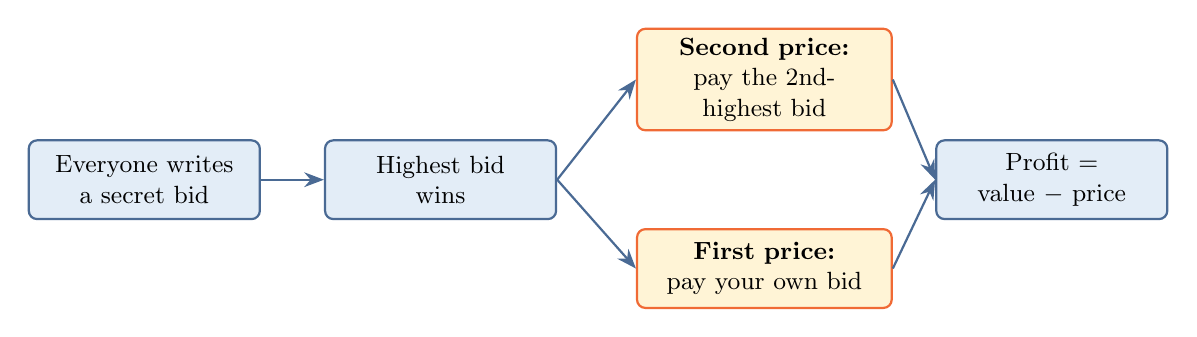
\begin{tikzpicture}[
      box/.style={draw=headblue, thick, fill=rowblue, rounded corners=3pt, align=center,
                  minimum height=10mm, text width=27mm, font=\small},
      pick/.style={draw=plotorange, thick, fill=good, rounded corners=3pt, align=center,
                   minimum height=10mm, text width=30mm, font=\small},
      go/.style={-{Stealth[length=2.5mm]}, thick, draw=headblue}]
    \node[box] (bids) {Everyone writes\\a secret bid};
    \node[box, right=8mm of bids] (win) {Highest bid\\wins};
    \node[pick, above right=1mm and 10mm of win] (sp) {\textbf{Second price:}\\pay the 2nd-highest bid};
    \node[pick, below right=1mm and 10mm of win] (fp) {\textbf{First price:}\\pay your own bid};
    \node[box, right=48mm of win] (profit) {Profit =\\value $-$ price};
    \draw[go] (bids) -- (win);
    \draw[go] (win.east) -- (sp.west);
    \draw[go] (win.east) -- (fp.west);
    \draw[go] (sp.east) -- (profit.west);
    \draw[go] (fp.east) -- (profit.west);
  \end{tikzpicture}
  \caption{One auction, step by step. The two auctions differ only in the orange step: which price the winner pays.}
  \label{fig:flow}
\end{figure}

We wrote everything in Python with \texttt{numpy}. Every number and plot in this report comes from that code.
All values are random numbers between 0 and 1 (uniform), unless we fix them.

Our answer in one line: \textbf{under second-price and VCG, telling the truth is always best. Under first price, it is not.}

% =====================================================================
\section{Part 1: Second-Price Auction}

\subsection{How we tested it}

Bidder~1 is ``us''. Our value $v$ is fixed to $0.2$, $0.5$ or $0.8$.
Bidder~2 is the rival. Its value is random. The rival plays one of three ways:

\begin{center}
\renewcommand{\arraystretch}{1.25}
\begin{tabular}{|l|l|}
\hline
\rowcolor{rowblue}\textbf{Rival strategy} & \textbf{What the rival bids} \\
\hline
(a) truthful & its own value \\ \hline
(b) half & half of its value \\ \hline
(c) random & a new random number; it ignores its value \\
\hline
\end{tabular}
\end{center}

We try every bid $b = 0.00, 0.01, \dots, 1.00$. For each bid we play \textbf{100{,}000 auctions} and take the average profit.

One small trick: every bid plays the \emph{same} 100{,}000 rival bids. This is fair, because each bid faces the same rivals.
It also removes random noise, so the best bid shows up clearly.
If two bids are exactly equal, we say the rival wins.

\subsection{A: Average profit for every bid}

\begin{figure}[h]
  \centering
  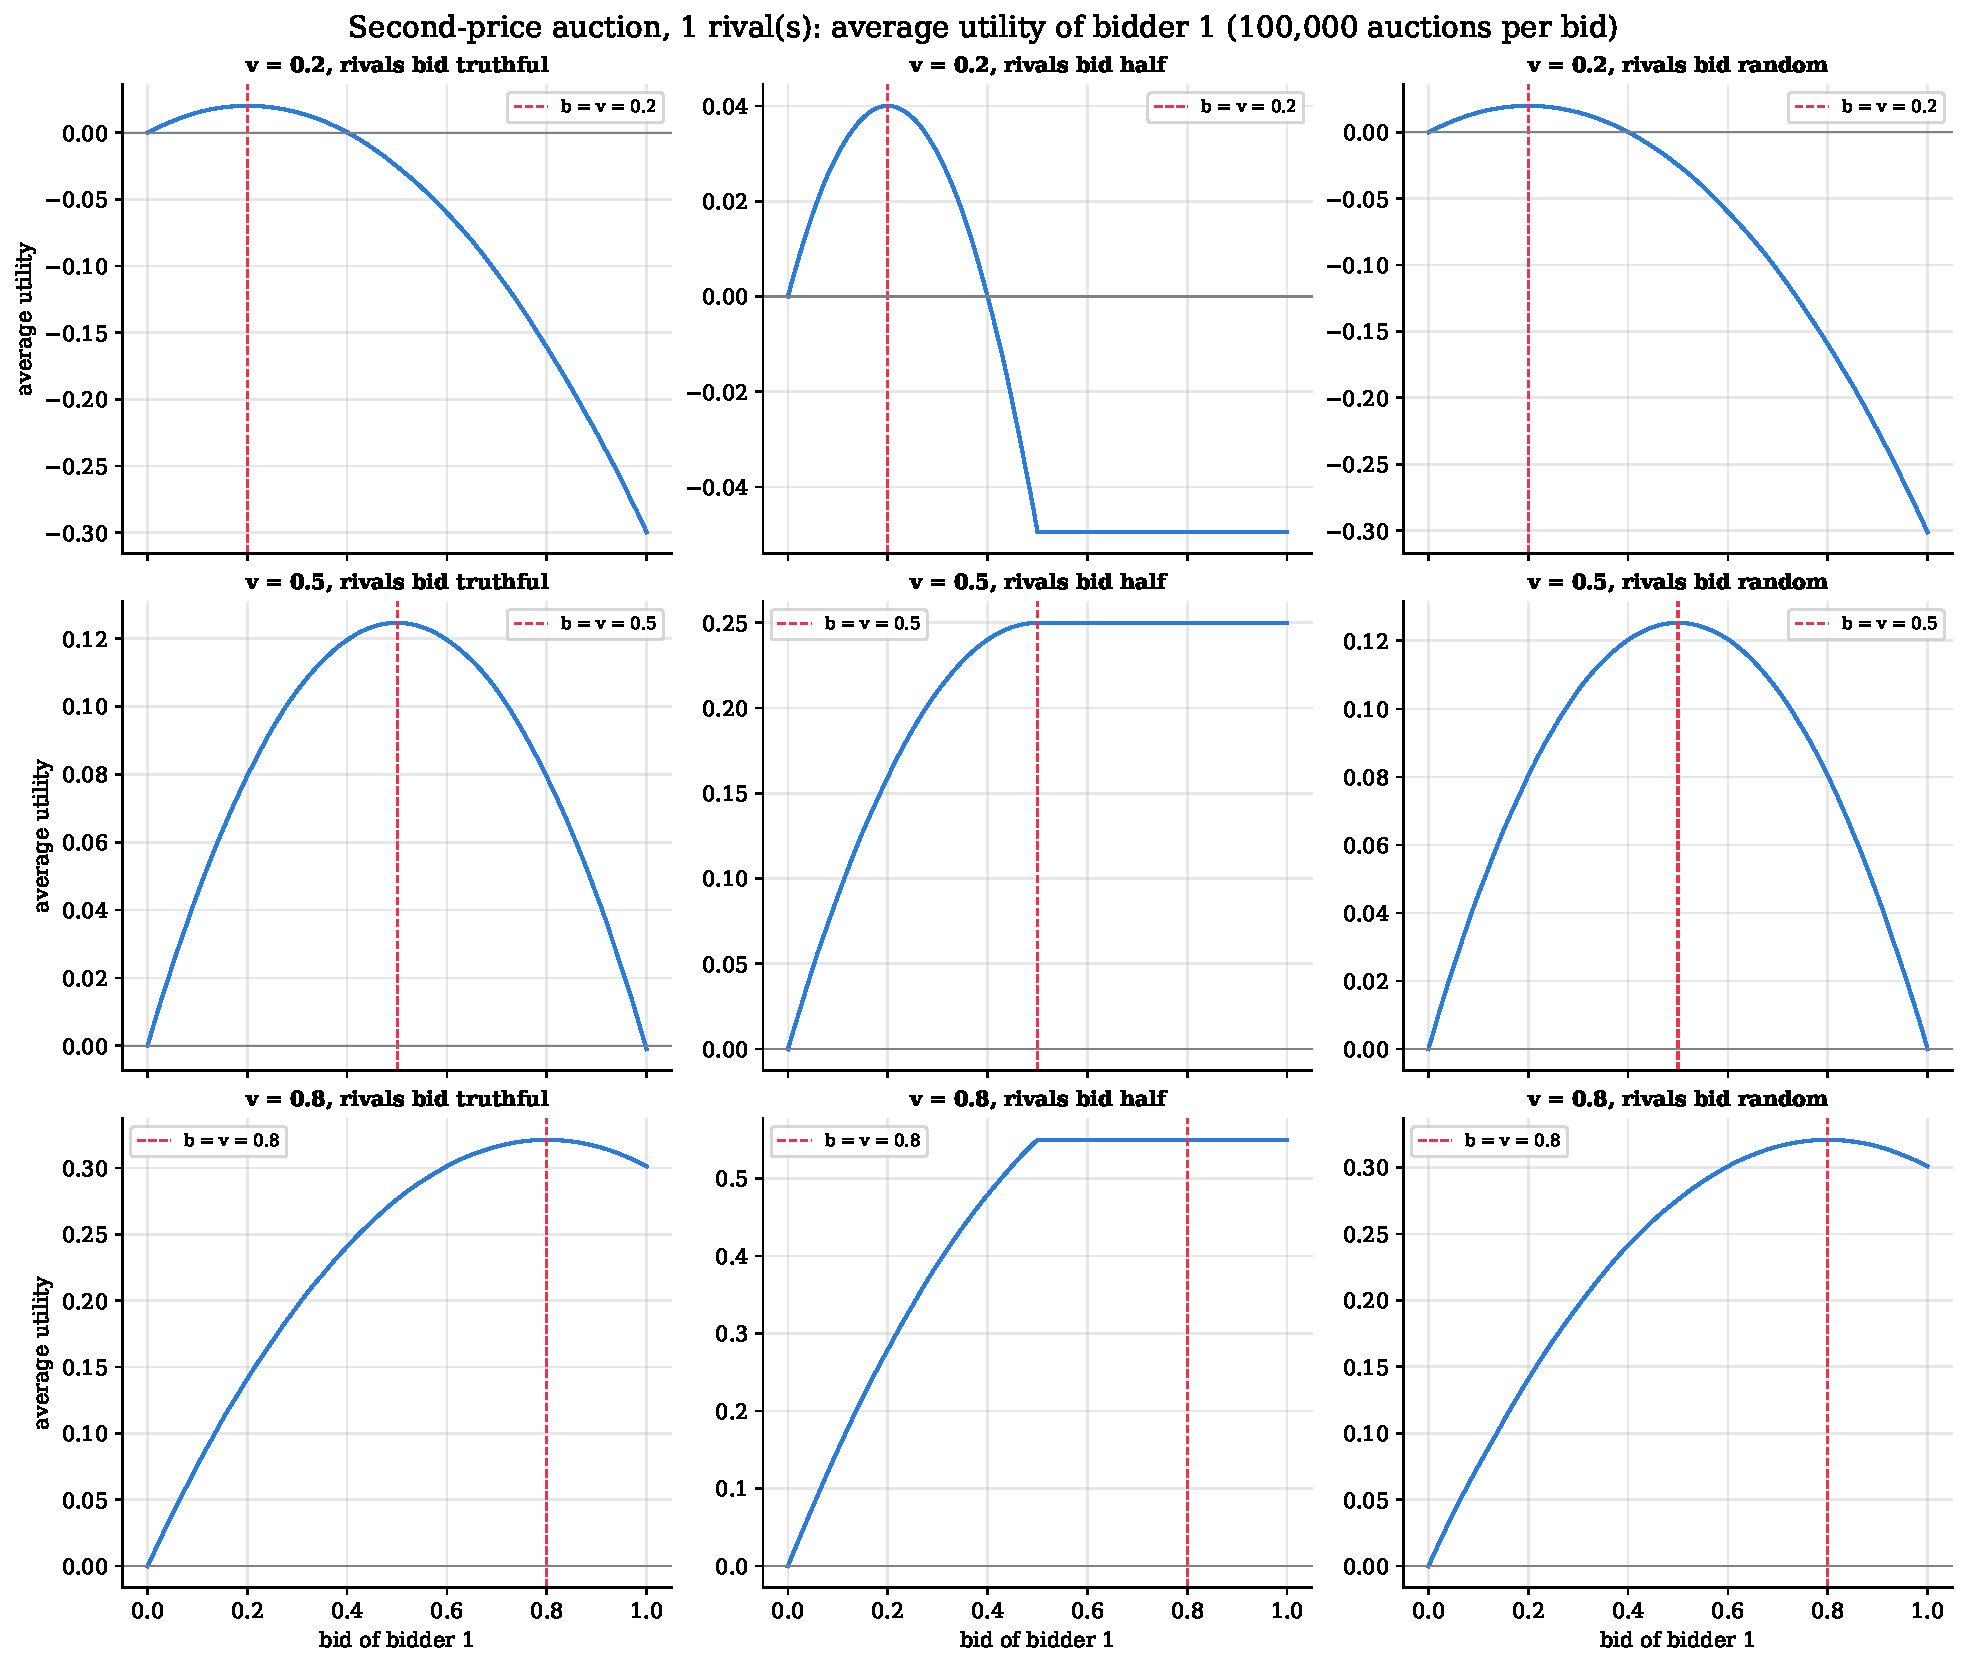
\includegraphics[width=\linewidth]{figures/part1A_1_rival.pdf}
  \caption{Part 1A, one rival. Each box is one value $v$ (rows) and one rival strategy (columns).
  The blue line is our average profit for each bid. The red dashed line is $b = v$.}
  \label{fig:1a}
\end{figure}

\textbf{What the plots show.} In all nine boxes, the highest point of the blue line sits on the red line, $b = v$.
So the best bid is our true value, no matter how the rival plays.

Why? Think of two mistakes (Figure~\ref{fig:mistakes}):

\begin{figure}[h]
  \centering
  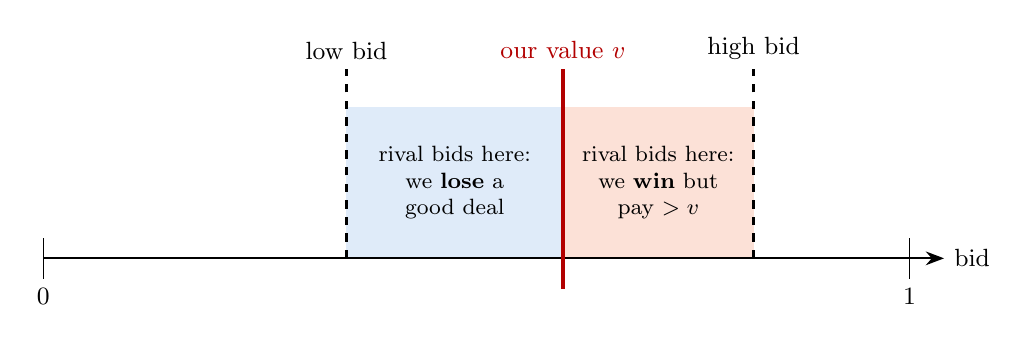
\begin{tikzpicture}[x=11cm, y=3.2cm]
    \fill[plotblue!15] (0.35,0) rectangle (0.6,0.6);
    \fill[plotorange!20] (0.6,0) rectangle (0.82,0.6);
    \draw[thick,-{Stealth}] (0,0) -- (1.04,0) node[right,font=\small] {bid};
    \foreach \x in {0,1} \draw (\x,0.08) -- (\x,-0.08) node[below,font=\small] {\x};
    \draw[very thick,red!70!black] (0.6,-0.12) -- (0.6,0.75) node[above,font=\small] {our value $v$};
    \draw[thick,dashed] (0.35,0) -- (0.35,0.75) node[above,font=\small] {low bid};
    \draw[thick,dashed] (0.82,0) -- (0.82,0.75) node[above,font=\small] {high bid};
    \node[align=center,font=\footnotesize] at (0.475,0.3) {rival bids here:\\we \textbf{lose} a\\good deal};
    \node[align=center,font=\footnotesize] at (0.71,0.3) {rival bids here:\\we \textbf{win} but\\pay $> v$};
  \end{tikzpicture}
  \caption{The two mistakes. If the rival's bid lands in the blue zone, a low bid loses an auction we wanted.
  If it lands in the orange zone, a high bid wins an auction we did not want. Bidding exactly $v$ makes both zones empty.}
  \label{fig:mistakes}
\end{figure}

\begin{itemize}
  \item \textbf{Bid too low.} Sometimes the rival bids between our bid and our value. We lose, but we could have won with a profit. That profit is gone.
  \item \textbf{Bid too high.} Sometimes the rival bids between our value and our bid. We win, but we pay more than the thing is worth. Our profit is below zero.
\end{itemize}
Bidding exactly $v$ avoids both mistakes. And our bid never changes the price we pay. The price is the rival's bid.

In the ``half'' column the line goes flat after $0.5$. A half-bidder never bids above $0.5$, so any bid above $0.5$ always wins at the same price.
Here $b = v$ is still a best bid. It is just not the only one.

\textbf{Do the plots help bidder~1 choose?} Yes. They give the same answer in every case: \emph{bid your value}.
Bidder~1 does not even need to know how the rival plays. This is what ``truthful bidding is a dominant strategy'' means.

\begin{table}[h]
\centering
\renewcommand{\arraystretch}{1.2}
\begin{tabular}{|c|c|c|c|}
\hline
\rowcolor{rowblue} \textbf{Our value $v$} & \textbf{Rival truthful} & \textbf{Rival half} & \textbf{Rival random} \\
\hline
0.2 & 0.020 & 0.040 & 0.020 \\ \hline
0.5 & 0.125 & 0.250 & 0.125 \\ \hline
0.8 & 0.321 & 0.550 & 0.321 \\
\hline
\end{tabular}
\caption{Average profit at $b = v$, one rival. In all nine cases this is the highest profit of any bid.
For a truthful rival, maths says the profit should be $v^2/2$, which is $0.02$, $0.125$ and $0.32$. Our numbers match.}
\end{table}

\subsection{B: The rival's bid is fixed}

Now the rival always bids the same number: $0.1$, $0.4$ or $0.9$. Nothing is random, so we just compute the profit.

There is only one thing to check: below the rival's bid we lose (profit $0$); above it we win and pay the rival's bid.
So we do not need a plot. Table~\ref{tab:1b} gives the result.

\begin{table}[h]
\centering
\renewcommand{\arraystretch}{1.2}
\begin{tabular}{|c|c|c|c|}
\hline
\rowcolor{rowblue} \textbf{Our value $v$} & \textbf{Rival bids 0.1} & \textbf{Rival bids 0.4} & \textbf{Rival bids 0.9} \\
\hline
0.2 & win, $+0.1$ & lose, $0$ & lose, $0$ \\ \hline
0.5 & win, $+0.4$ & win, $+0.1$ & lose, $0$ \\ \hline
0.8 & win, $+0.7$ & win, $+0.4$ & lose, $0$ \\
\hline
\end{tabular}
\caption{Part 1B. What happens when we bid $b = v$ against a fixed rival bid. Our code tried every bid from 0 to 1;
in all nine cases no bid gave more profit than $b = v$.}
\label{tab:1b}
\end{table}

\begin{itemize}
  \item If our value is \textbf{above} the rival's bid, winning is good. Bidding $v$ wins.
  \item If our value is \textbf{below} the rival's bid, winning is bad (we would pay too much). Bidding $v$ loses, which is right.
\end{itemize}

So in all nine cases, $b = v$ gives the highest profit. Truthful bidding works against \emph{every} rival bid.

\subsection{C: Two rivals}

Now there are two rivals, bidder~2 and bidder~3. Both use the same strategy, and both have random values.
The price is now the \emph{higher} of the two rival bids. We repeated parts A and B.
(The assignment says ``repeat parts A and C''; we read this as A and B.)

\begin{figure}[h]
  \centering
  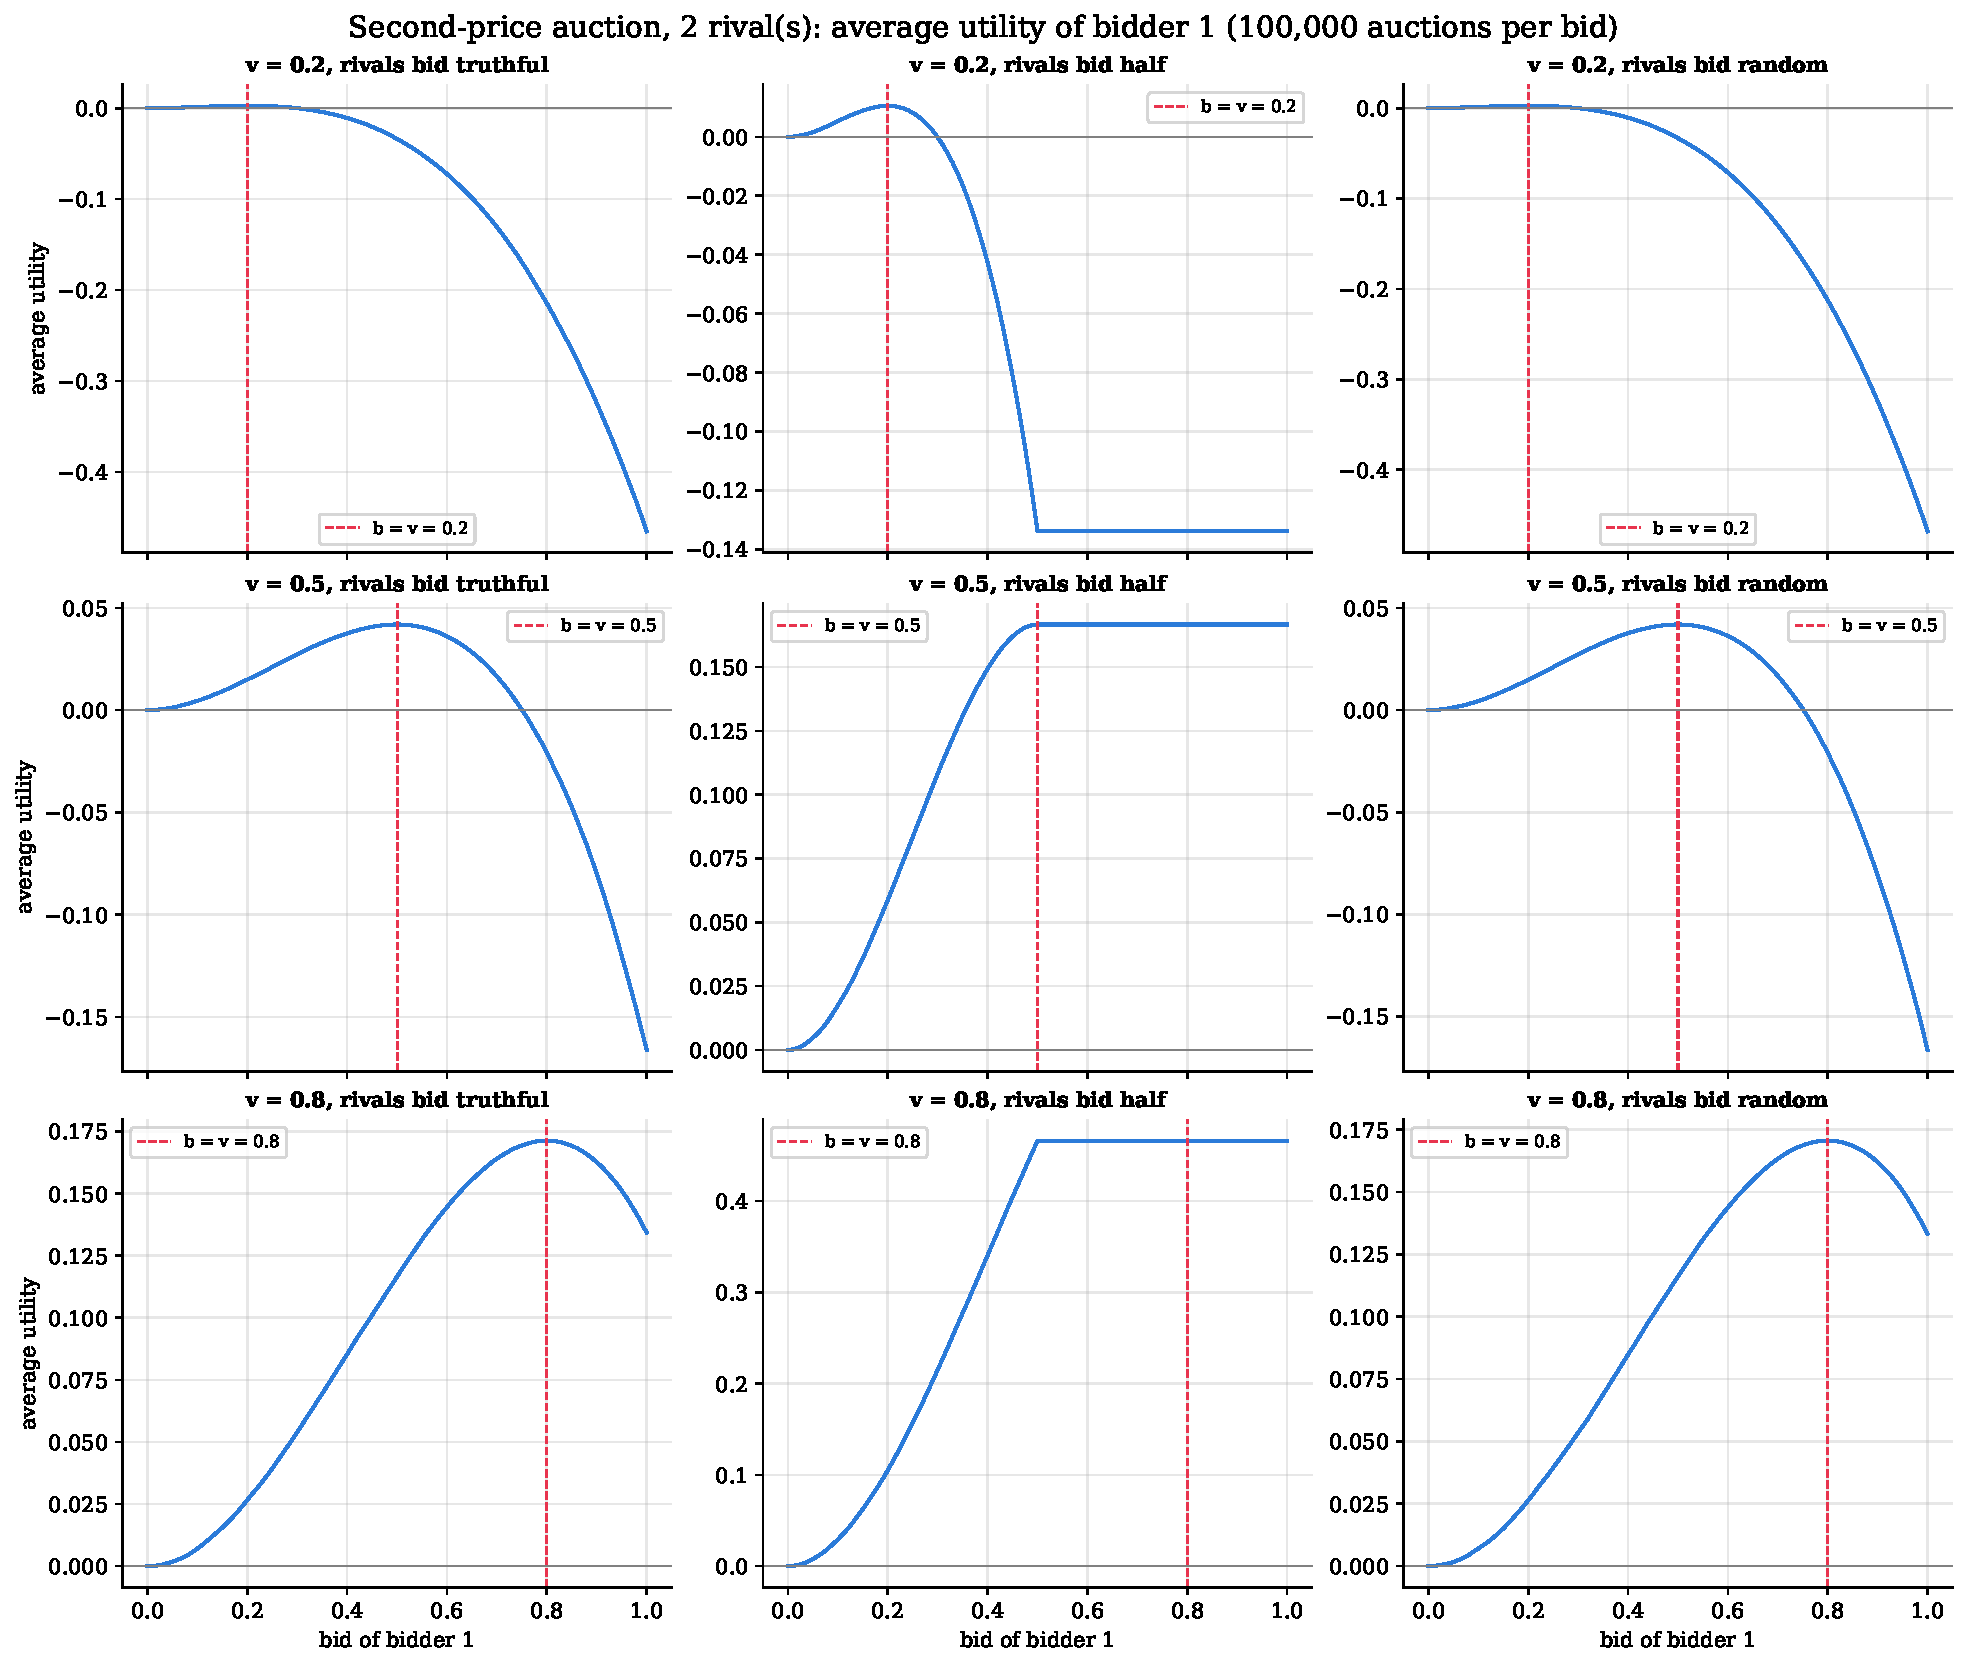
\includegraphics[width=\linewidth]{figures/part1A_2_rival.pdf}
  \caption{Part 1C (repeat of A), two rivals. The best bid is still $b = v$ in all nine cases.}
  \label{fig:1c}
\end{figure}

For the repeat of part~B, both rivals use the same fixed bid. The higher rival bid is then just that bid,
so the results are exactly Table~\ref{tab:1b} again, and $b = v$ is again best in all nine cases.

Profits are smaller, because with two rivals it is harder to win. But the shape of the answer does not change.
The reason from part~A still holds: our bid only decides \emph{if} we win, never \emph{how much} we pay.

% =====================================================================
\section{Part 2: First-Price Auction}

\subsection{How we tested it}

Now the winner pays their \textbf{own} bid. There are $n$ bidders, for $n = 2, 3, 4$. Everyone's value is random.

The other $n-1$ bidders play the known best strategy (the \emph{equilibrium}): they bid
\[
\text{bid} = \frac{n-1}{n} \times \text{value}.
\]
We (bidder~1) bid $k \times v$, and try $k = 0.1, 0.2, \dots, 2.0$. For each $k$ we play 100{,}000 auctions.

\subsection{Results}

\begin{figure}[h]
  \centering
  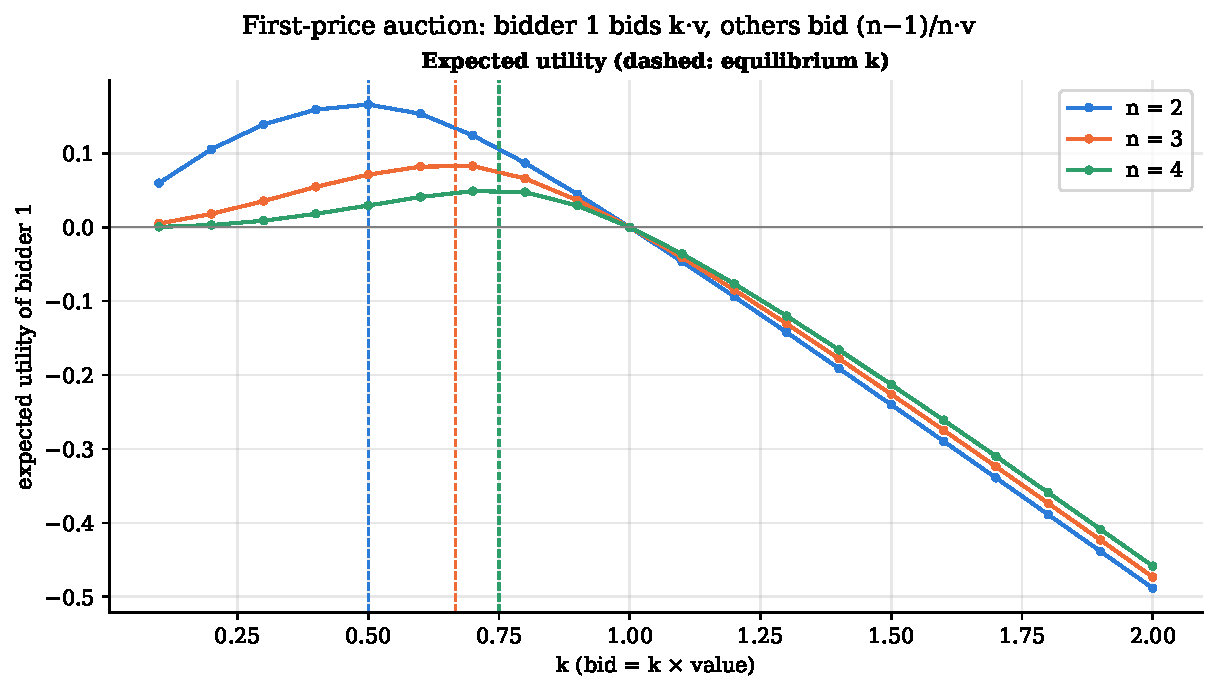
\includegraphics[width=0.75\linewidth]{figures/part2_first_price.pdf}
  \caption{Part 2. Our average profit for each $k$. Each curve peaks near its dashed line, the equilibrium $k = (n-1)/n$.
  At $k = 1$ (bid the truth) every curve is at $0$.}
  \label{fig:2}
\end{figure}

\begin{table}[h]
\centering\small
\renewcommand{\arraystretch}{1.2}
\begin{tabular}{|c|c|c|c|c|c|}
\hline
\rowcolor{rowblue} $\boldsymbol{n}$ & \textbf{Equilibrium $k$} & \textbf{Best $k$ on grid} & \textbf{Best profit} & \textbf{Could pay less} & \textbf{Average overpay} \\
\hline
2 & 0.50 & 0.5 & 0.166 & 100\% & 0.166 \\ \hline
3 & 0.67 & 0.7 & 0.083 & 100\% & 0.170 \\ \hline
4 & 0.75 & 0.7 & 0.049 & 100\% & 0.149 \\
\hline
\end{tabular}
\caption{Part 2, 100{,}000 auctions per $k$. ``Average overpay'' is the winning bid minus the second-highest bid, at the $k$ closest to equilibrium.}
\label{tab:2}
\end{table}

\textbf{Bidding the truth is now bad.} At $k = 1$ (bid your value), the profit is exactly $0$. You win, but you pay all of your value.
Above $k = 1$ the profit is below zero.

\textbf{The best $k$ is below 1.} It matches the equilibrium $(n-1)/n$: $0.5$ for two bidders, about $0.67$ for three, $0.75$ for four.
For $n = 4$ the grid has no $0.75$, so the best grid point is $0.7$ (profit $0.0489$, just above $0.0475$ at $0.8$).
This shows that when everyone else plays the equilibrium, we cannot do better by moving away from it.

\textbf{More bidders means bid closer to your value.} With more rivals, a low bid loses more often, so you must bid higher.

\textbf{The winner could always have paid less.} In 100\% of auctions, the winner's bid was above the second-highest bid.
The winner could have bid just above the second bid, still won, and kept the difference (about $0.15$ to $0.17$ on average).
This is the big problem with first price: you always pay more than you needed to, so everyone tries to guess the others and bids low.
In second price this cannot happen, because the winner already pays exactly the second bid.

% =====================================================================
\section{Part 3: VCG for the Cheapest Path}

\subsection{The problem}

We want to send something from A to F. Each road (edge) has an owner. The owner knows what the road really costs, but we do not.
We ask each owner to tell us their cost. Then we pick the cheapest path and pay the owners.

Owners could lie to get more money. \textbf{VCG} pays them in a way that makes lying useless.

\begin{figure}[h]
  \centering
  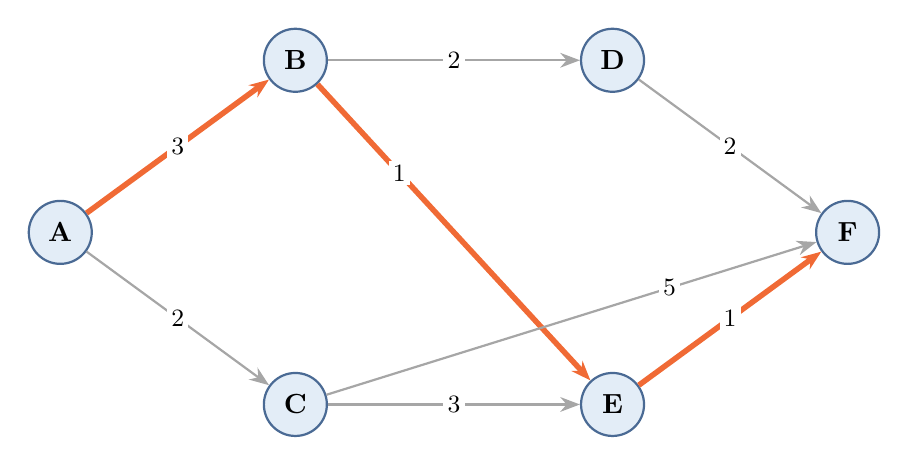
\begin{tikzpicture}[
      node distance=1.6cm and 2.4cm,
      town/.style={circle, draw=headblue, thick, fill=rowblue, minimum size=8mm, font=\bfseries},
      road/.style={-{Stealth[length=2.5mm]}, thick, draw=gray!70},
      best/.style={-{Stealth[length=2.5mm]}, line width=2pt, draw=plotorange},
      cost/.style={font=\small, fill=white, inner sep=1.5pt}]
    \node[town] (A) {A};
    \node[town, above right=of A] (B) {B};
    \node[town, below right=of A] (C) {C};
    \node[town, right=3.2cm of B] (D) {D};
    \node[town, right=3.2cm of C] (E) {E};
    \node[town, below right=of D] (F) {F};
    \draw[best] (A) -- node[cost] {3} (B);
    \draw[road] (A) -- node[cost] {2} (C);
    \draw[road] (B) -- node[cost] {2} (D);
    \draw[best] (B) -- node[cost, pos=0.3] {1} (E);
    \draw[road] (C) -- node[cost] {3} (E);
    \draw[road] (C) -- node[cost, pos=0.7] {5} (F);
    \draw[road] (D) -- node[cost] {2} (F);
    \draw[best] (E) -- node[cost] {1} (F);
  \end{tikzpicture}
  \caption{The road network from Figure 7.3 of the book. Numbers are the true costs. The cheapest path, A$\to$B$\to$E$\to$F (cost $3+1+1=5$), is in orange.}
  \label{fig:graph}
\end{figure}

\subsection{How VCG pays}

For each road, ask two questions (Figure~\ref{fig:vcgflow}):
\begin{enumerate}
  \item How much would the cheapest path cost \textbf{if this road did not exist}?
  \item How much do the \textbf{other} roads on the chosen path cost?
\end{enumerate}
The road is paid the first number minus the second.

\begin{figure}[h]
  \centering
  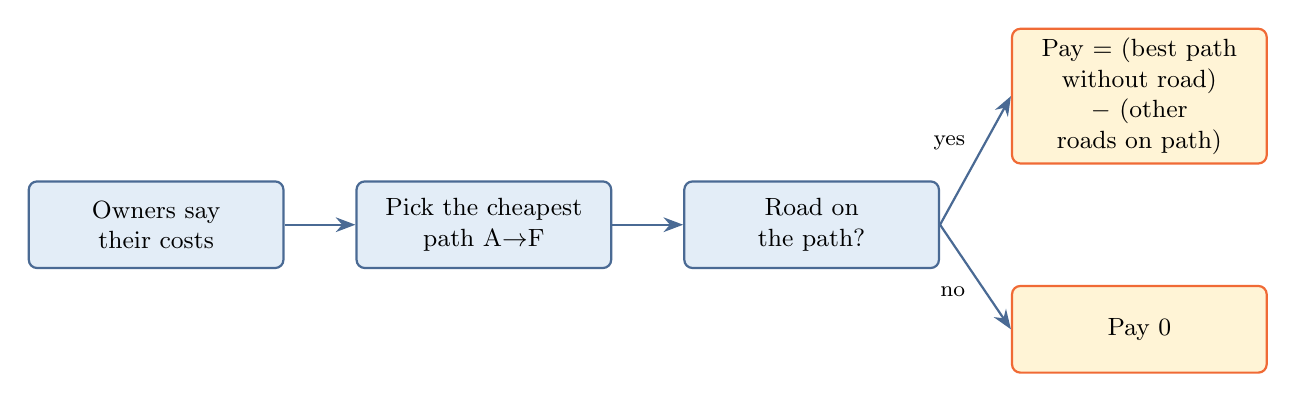
\begin{tikzpicture}[
      box/.style={draw=headblue, thick, fill=rowblue, rounded corners=3pt, align=center,
                  minimum height=11mm, text width=30mm, font=\small},
      pay/.style={draw=plotorange, thick, fill=good, rounded corners=3pt, align=center,
                  minimum height=11mm, text width=30mm, font=\small},
      go/.style={-{Stealth[length=2.5mm]}, thick, draw=headblue}]
    \node[box] (ask) {Owners say\\their costs};
    \node[box, right=9mm of ask] (path) {Pick the cheapest\\path A$\to$F};
    \node[box, right=9mm of path] (q) {Road on\\the path?};
    \node[pay, above right=2mm and 9mm of q] (yes) {Pay = (best path\\without road) $-$ (other\\roads on path)};
    \node[pay, below right=2mm and 9mm of q] (no) {Pay $0$};
    \draw[go] (ask) -- (path);
    \draw[go] (path) -- (q);
    \draw[go] (q.east) -- node[above left, font=\footnotesize] {yes} (yes.west);
    \draw[go] (q.east) -- node[below left, font=\footnotesize] {no} (no.west);
  \end{tikzpicture}
  \caption{How VCG decides each payment. Notice that a road's own claimed cost is not used in its payment;
  it only decides if the road is on the path.}
  \label{fig:vcgflow}
\end{figure}
In simple words: a road is paid for how much \emph{worse} things would be without it.
A road that is not on the path changes nothing, so it is paid $0$.

\begin{table}[h]
\centering\small
\renewcommand{\arraystretch}{1.25}
\begin{tabular}{|c|c|c|c|c|}
\hline
\rowcolor{rowblue} \textbf{Road} & \textbf{Best path without it} & \textbf{Other roads on ABEF} & \textbf{Payment} & \textbf{Profit} \\
\hline
AB & ACEF $= 6$ & BE $+$ EF $= 2$ & $6 - 2 = \mathbf{4}$ & $4 - 3 = 1$ \\ \hline
BE & ACEF $= 6$ & AB $+$ EF $= 4$ & $6 - 4 = \mathbf{2}$ & $2 - 1 = 1$ \\ \hline
EF & ABDF $= 7$ & AB $+$ BE $= 4$ & $7 - 4 = \mathbf{3}$ & $3 - 1 = 2$ \\ \hline
others & no change & -- & $\mathbf{0}$ & $0$ \\
\hline
\end{tabular}
\caption{VCG payments from our code. They match the book: AB is paid 4, BE is paid 2, EF is paid 3, every other road 0.}
\label{tab:vcg}
\end{table}

Our code finds the path with Dijkstra's shortest-path method, and runs it again with each road removed.
When two paths cost the same, it picks the one that comes first in alphabetical order.

\subsection{Does lying help?}

We picked one road \textbf{on} the path (AB, true cost 3) and one road \textbf{off} the path (AC, true cost 2).
Each one tells every cost from $0$ to $10$ in steps of $0.5$. All other roads tell the truth.

\begin{figure}[h]
  \centering
  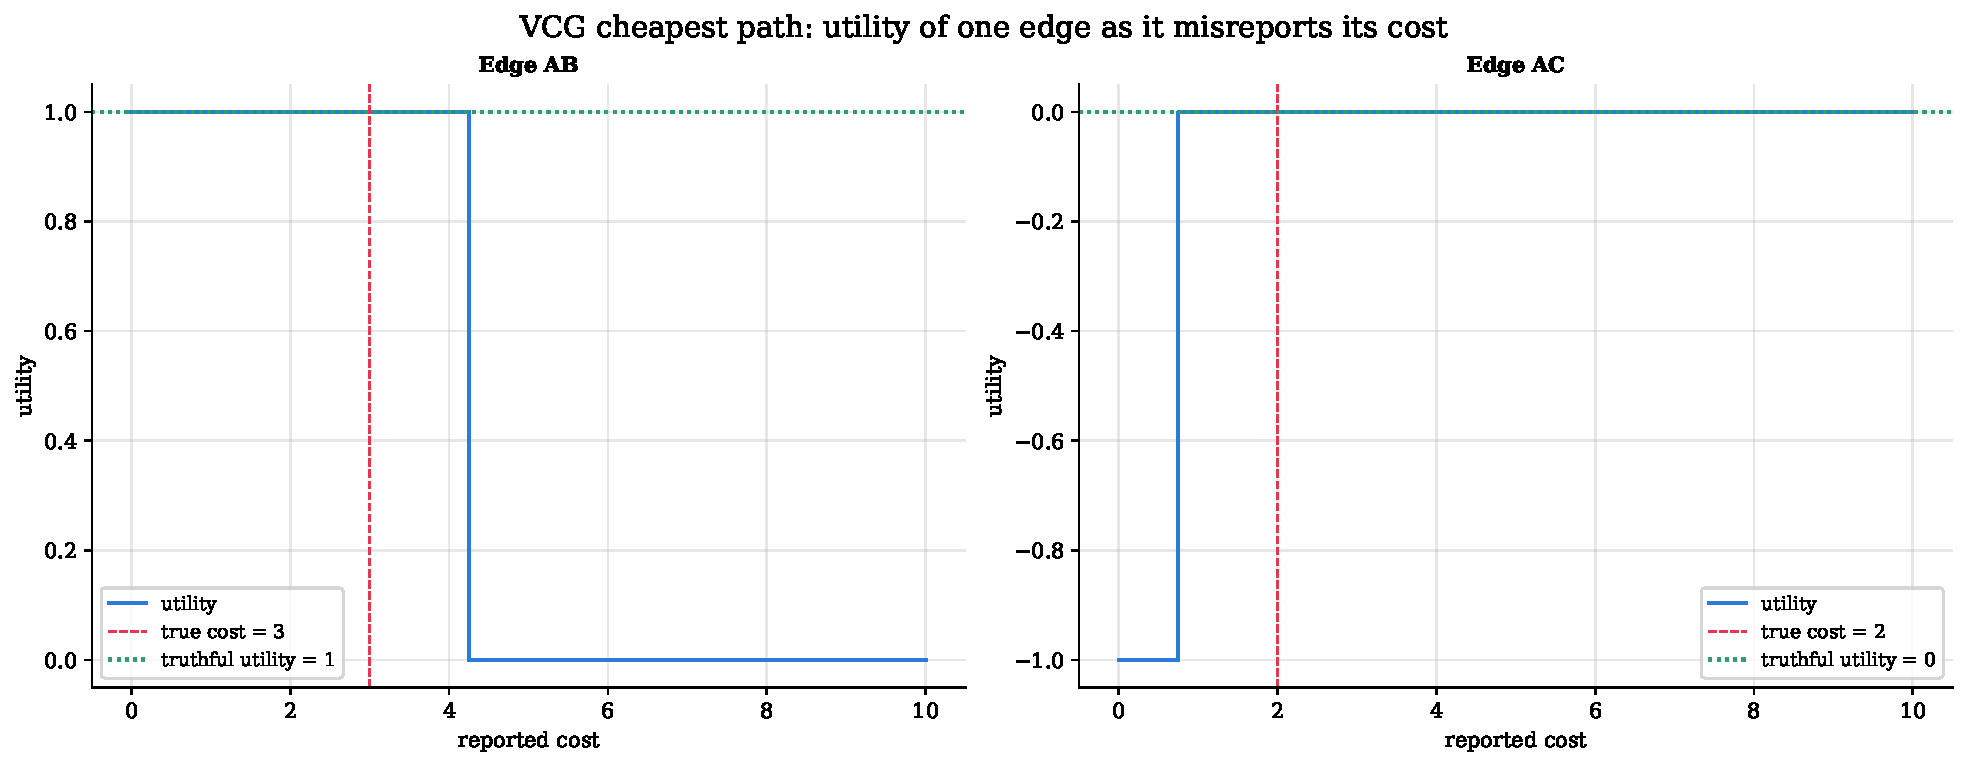
\includegraphics[width=\linewidth]{figures/part3_vcg_misreport.pdf}
  \caption{Part 3. The profit of road AB (left) and road AC (right) for every cost it could claim.
  The red line is the true cost. The green line is the profit from telling the truth.}
  \label{fig:3}
\end{figure}

\textbf{Road AB (on the path).} Telling the truth gives profit $1$.
\begin{itemize}
  \item Claiming any cost up to $4$ changes nothing. AB stays on the path and is still paid $4$. The payment does not depend on what AB says.
  \item Claiming more than $4$ makes the path A$\to$C$\to$E$\to$F cheaper. AB loses the job and its profit drops to $0$.
\end{itemize}

\textbf{Road AC (off the path).} Telling the truth gives profit $0$.
\begin{itemize}
  \item Claiming a cost of $1$ or more changes nothing. AC stays off the path.
  \item Claiming less than $1$ (here $0$ or $0.5$) puts AC on the path. AC is paid $5 - 4 = 1$, but the road really costs $2$. Its profit is $-1$. It wins the job and loses money.
\end{itemize}

So \textbf{no lie ever gives more profit than the truth}. This is the same idea as in the second-price auction.
What you say only decides \emph{if} you are picked. It never changes \emph{how much} you are paid.
In fact, the second-price auction is just VCG for selling one item.

% =====================================================================
\section{Conclusion}

\begin{center}
\renewcommand{\arraystretch}{1.3}
\begin{tabularx}{0.95\linewidth}{|l|l|X|}
\hline
\rowcolor{rowblue} \textbf{Rule} & \textbf{Best strategy} & \textbf{Why} \\
\hline
Second price & Bid your true value & You pay the next bid, so your bid only decides if you win. Works for any rival and for two rivals. \\ \hline
First price & Bid less: $\frac{n-1}{n}\times$ value & You pay your own bid, so bidding the truth gives zero profit. The winner always overpays. \\ \hline
VCG & Tell your true cost & You are paid for how much you help, not for what you say. Lying can only lose the job or lose money. \\
\hline
\end{tabularx}
\end{center}

The lesson: a good \textbf{mechanism} makes the honest choice also the best choice.
Second price and VCG do this. First price does not, so people must guess and shade their bids.
Our simulations show this with numbers: in every test, the truthful bid or report was never beaten under second price or VCG.

\end{document}
